Los resultados presentados en esta sección se obtuvieron mediante un análisis experimental automatizado. Para ello, se implementaron dos versiones del algoritmo de distancia de edición: una utilizando fuerza bruta y otra mediante programación dinámica. Los tiempos de ejecución y las operaciones fueron registrados para varios conjuntos de pruebas.\\

\noindent Todos los gráficos y tablas que se muestran a continuación fueron generados utilizando un programa en Python. Este programa automatiza el análisis de datos, permitiendo la ejecución repetible de los experimentos y la visualización de los resultados en forma de gráficos comparativos y tablas de operaciones. Los archivos utilizados para la generación de estos resultados están disponibles, lo que asegura la reproducibilidad de los análisis al ejecutar los scripts provistos.\\

\noindent En la \cref{cantOpe} se observa la comparación entre los resultados de Fuerza Bruta y Programación Dinámica en términos de cantidad de operaciones. Se puede apreciar que los algoritmos producen resultados idénticos en todos los casos de prueba. Esto confirma que la implementación de ambos enfoques es correcta y que generan la misma distancia de edición, independientemente del método utilizado.

\begin{figure}[H]
    \centering
    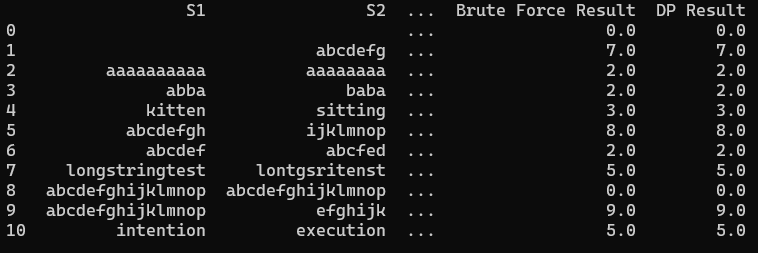
\includegraphics[width=\textwidth]{images/cantOpe.png}
    \caption{Comparación cantidad de operaciones BF y DP.}
    \label{cantOpe}
\end{figure}

\noindent La \cref{times} muestra los tiempos promedio registrados para el paradigma de Fuerza Bruta y la diferencia de este con el de Programación Dinámica. Es posible notar grandes diferencias en favor de la Fuerza Bruta en las entradas 5, 7 y 9. Y diferencias significativas a favor de la Porgramación Dinámica en las entradas 0, 6 y 8; lo que destaca su superioridad en cadenas idénticas (0 y 8).

\begin{figure}[H]
    \centering
    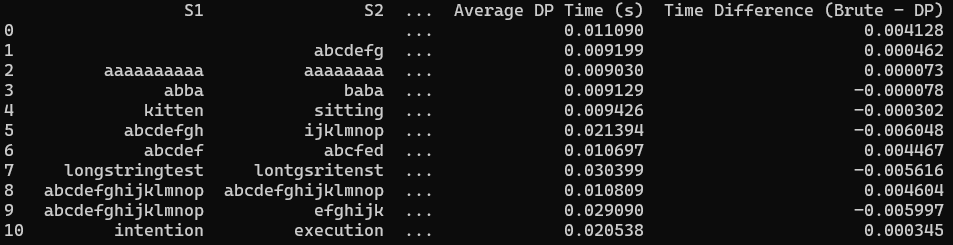
\includegraphics[width=\textwidth]{images/times.png}
    \caption{Tiempos promedio por entrada.}
    \label{times}
\end{figure}

\noindent Se generó también una comparativa gráfica de tiempos \cref{compTimes}, donde sorprendentemente, los resultados muestran que, en varios casos, la Programación Dinámica (línea naranja) presentó tiempos de ejecución más altos que la Fuerza Bruta (línea azul). Este comportamiento es inesperado, ya que, teóricamente, DP debería ser más eficiente debido a su optimización de subproblemas recurrentes, mientras que FB explora todas las posibles soluciones.\\

Se plantean varias hipótesis para explicar este comportamiento:

    \begin{itemize}
        \item La implementación de DP puede estar introduciendo sobrecargas innecesarias que afectan su rendimiento.
        \item En casos con cadenas cortas, la sobrecarga computacional de DP podría ser mayor que el beneficio obtenido por su eficiencia en la solución de subproblemas.
        \item Es posible que el entorno de experimentación o la manera en que se realizaron las mediciones pueda haber introducido sesgos que favorezcan a FB.
    \end{itemize}

\begin{figure}[H]
    \centering
    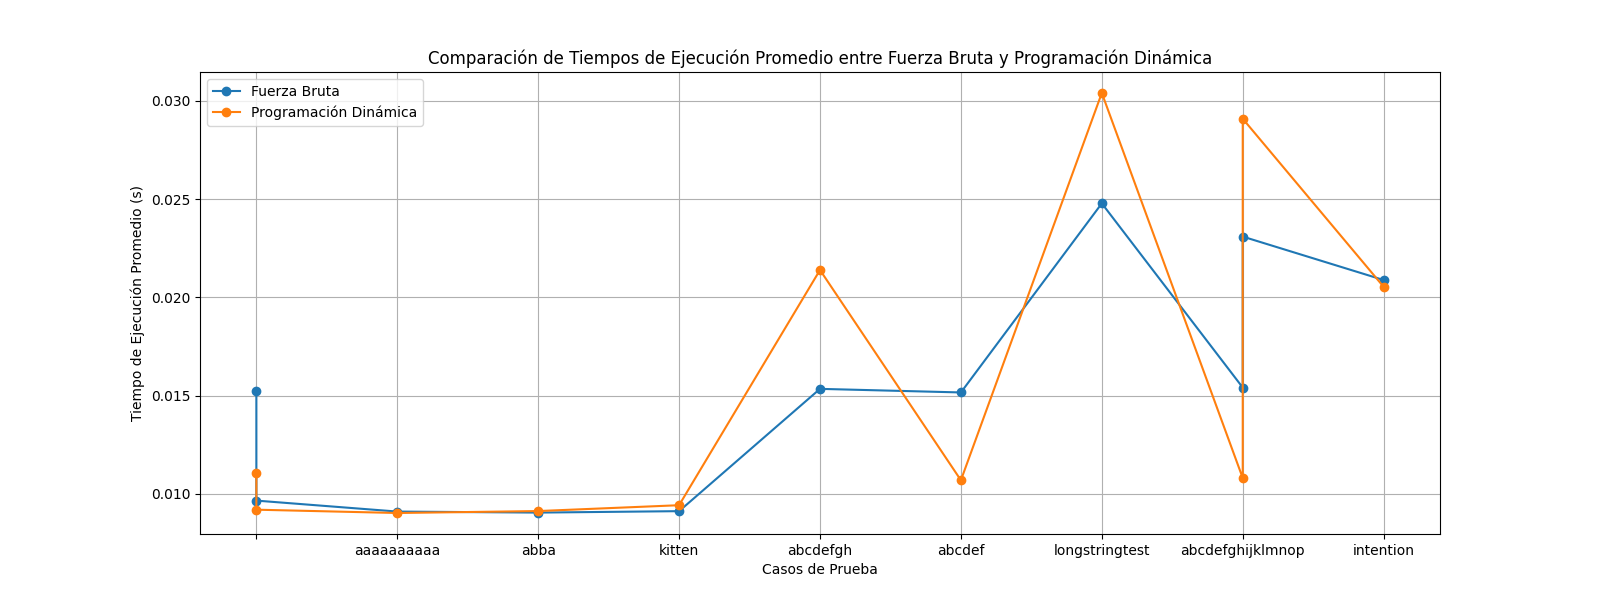
\includegraphics[width=\textwidth]{images/comparison_execution_times.png}
    \caption{Comparación de tiempos BF y DP.}
    \label{compTimes}
\end{figure}
\newpage

\noindent La Figura \cref{boxplot} muestra la distribución de los tiempos de ejecución de ambos algoritmos, excluyendo valores atípicos para mayor claridad. Se puede observar que la mediana de los tiempos de ejecución de Fuerza Bruta es ligeramente superior a la de Programación Dinámica, lo que a primera vista parece indicar que la implementación de DP es más eficiente en promedio. Sin embargo, hay ciertos detalles que merecen atención:

\begin{enumerate}
    \item \textbf{Mayor variabilidad en DP:} La distribución de tiempos de DP muestra una mayor dispersión. Esto sugiere que DP es más sensible a las características de las cadenas de entrada, ya que su rendimiento parece fluctuar considerablemente entre diferentes casos.
    
    \item \textbf{Máximos más altos en DP:} Aunque los tiempos promedio de ambos algoritmos son comparables, Programación Dinámica presenta valores máximos de tiempo más elevados que Fuerza Bruta.
    
    \item \textbf{Tiempos más consistentes en FB:} En contraste, Fuerza Bruta presenta una menor variabilidad en sus tiempos, lo que refleja su naturaleza más predecible y lineal, a pesar de su complejidad exponencial en teoría.
\end{enumerate}

Este gráfico nos indica que, aunque la teoría sugiere que DP debería ser más eficiente que FB, en la práctica esto no siempre ocurre, dependiendo de la implementación y las características de los datos de entrada.

\begin{figure}[H]
    \centering
    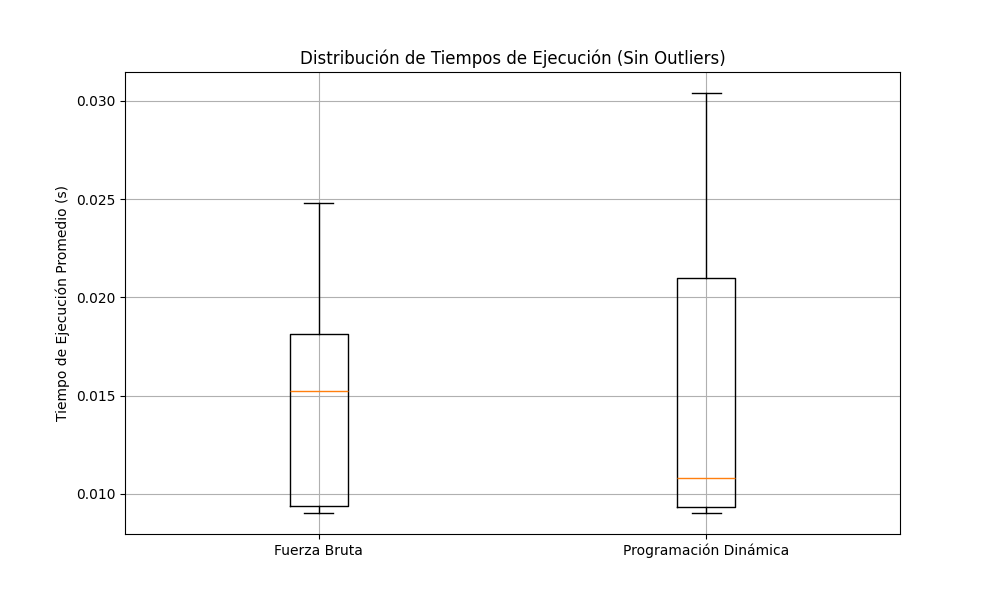
\includegraphics[width=\textwidth]{images/execution_time_distribution.png}
    \caption{Distribución de tiempos de ejecución (boxplot)}
    \label{boxplot}
\end{figure}
\newpage

\noindent En la figura \cref{timeVsLen}, se presenta la comparación entre los tiempos de ejecución promedio de los algoritmos de Fuerza Bruta y Programación Dinámica en función de la longitud de las cadenas de entrada. Los resultados muestran un comportamiento inesperado en varios aspectos clave:

\begin{enumerate}
    \item \textbf{Rendimiento para cadenas cortas:} En los primeros casos de prueba (longitudes menores a 8), la Programación Dinámica es consistentemente más rápida que la Fuerza Bruta, lo cual es acorde con la complejidad teórica esperada. Sin embargo, las diferencias de tiempo entre ambos algoritmos son mínimas, con variaciones de milisegundos.
    
    \item \textbf{Ineficiencia creciente de Programación Dinámica:} A partir de cadenas con longitud 8 en adelante, la Programación Dinámica comienza a exhibir tiempos de ejecución significativamente más altos que la Fuerza Bruta, especialmente para las longitudes 13.5 y 11.5. Este comportamiento es inesperado, dado que DP tiene una complejidad teórica inferior a la de BF, sugiriendo sugiere que existen posibles ineficiencias en la implementación de DP.
    
    \item \textbf{Estabilidad de Fuerza Bruta en cadenas largas:} Contrario a la expectativa de un incremento exponencial en los tiempos de Fuerza Bruta, el gráfico revela que este algoritmo mantiene una curva de crecimiento más estable, e incluso logra tiempos menores que DP en varios casos con cadenas largas.
\end{enumerate}

\begin{figure}[H]
    \centering
    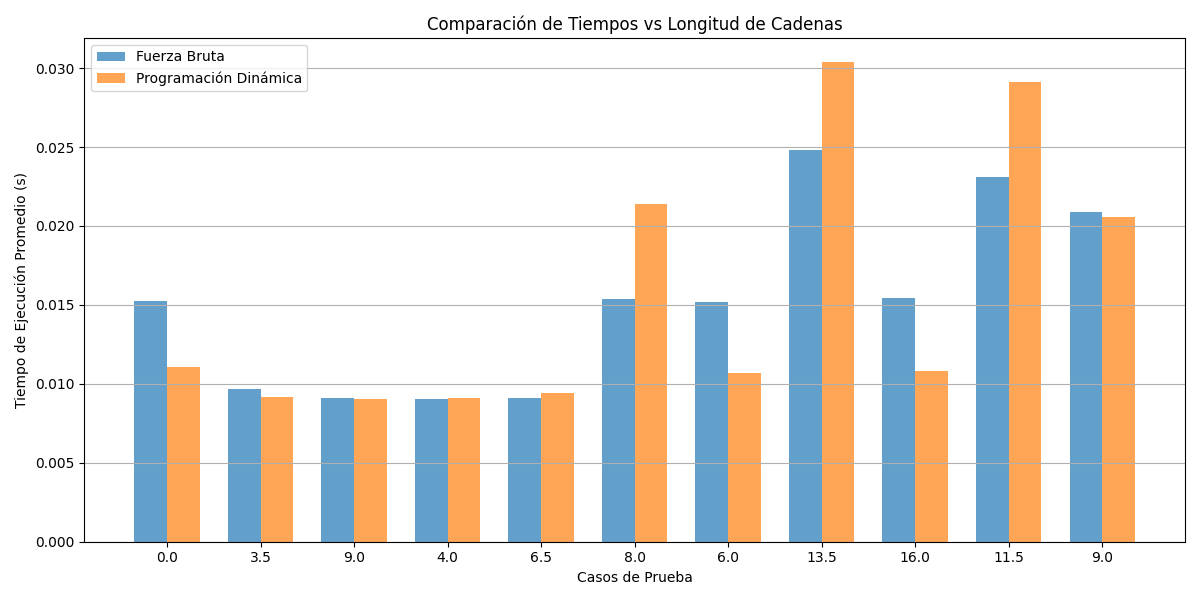
\includegraphics[width=\textwidth]{images/execution_times_vs_length.png}
    \caption{Comparación tiempos de ejecución vs longitud de cadenas BF y DP.}
    \label{timeVsLen}
\end{figure}